\documentclass[12pt,a4paper]{article}
\usepackage[latin1]{inputenc}
\usepackage{float}
\usepackage{amsmath}
\usepackage{amsfonts}
\usepackage{amssymb}
\usepackage{graphicx}
\usepackage[hidelinks]{hyperref}
\usepackage{changepage}
\usepackage{subfig}
\usepackage{placeins}



\author{Davide Cocco - 944122\\
	Marco Gasperini - 944922}
\date{A.Y. 2019/2020 - Prof. Di Nitto Elisabetta}


\title{
	\textbf{\Huge{SafeStreets}} \\
	\large Design Document
}

\begin {document}

	\begin{figure}
		\centering
		
\includegraphics[width=1.0\linewidth]{Images/polimi.jpg}
	\end{figure}

	\maketitle
	\newpage
	\tableofcontents
	\newpage

\section{INTRODUCTION}
\subsection{Purpose}
This \texttt{Design Document (DD)} for the SafeStreets software will provide a functional description of the system by describing its architecture. 
It will eventually by used by the development team as a blueprint to guide the engineering of the application.
\subsection{Scope}
The main objective of the S2B will be assisting (thus not substituting) authorities and officers in handling traffic violations though a crowd-sourced platform in which civilians can participate. 
A mobile application will allow users, both civilians and officers, to report violations through the use of the camera and the GPS, sending the data to authorities who will process such reports. 
Law enforcement will be aided by a data mining system which will produce relevant data about the registered violations, and the S2B will be able to automatically compile a ticket and send it to
the municipality's VLA as soon as an officer personally convalidates a violation.
\subsection{Definitions, Acronyms, Abbreviations}
\subsubsection{Definitions}
\begin{itemize}
\item \texttt{Violation | Offence:} we will strictly refer to any kind of static traffic violation, especially parking violations. 
\item \texttt{Authority:} a law enforcement authority which is manages traffic violations, it could be the local police, the traffic wardens etc. We will refer with this term also to the personnel which operates the web application in the authorities' headquarters.
\item \texttt{User:} refers to the users of the mobile application, that is officers and civilians.
\end{itemize}
\subsubsection{Acronyms}
\begin{itemize}
\item \texttt{S2B:} software to be.
\item \texttt{HFVZ:} high violation frequency zone.
\item \texttt{GPS:} Global Positioning System.
\item \texttt{GDPR:} General Data Protection Regulation.
\item \texttt{DW:} data warehouse.
\item \texttt{VLA:} Vehicle Licensing Authority.
\item \texttt{RACS:} Reliable Array of Cloned Services.
\item \texttt{RAPS:} Reliable Array of Partitioned Services.
\item \texttt{GUI:} Graphical User Interface.
\item \texttt{DMZ:} Demilitarized zone.
\item \texttt{ADS:} Application and Data server of the authorities.
\item \texttt{API:} Application Programming Interface.
\end{itemize}
\subsubsection{Abbreviations}
\begin{itemize}
	\item {[Gn]}: n-goal.
	\item {[Rn]}: n-requirment.
	\item {[Dn]}: n-domain assumption
	\item {App}: application.
\end{itemize}
\subsection{Revision History}
\subsection{Reference Documents}
\subsection{Document Structure}
\begin{itemize}
\item \textbf{Introduction}: includes the purpose and scope of the document along with some relevant definitions and acronyms used throughout the document.
\item \textbf{Architectural design}: this section is focused on the main components used for this system and the relationship between them, providing information about their
deployment and how they operate. it also focuses on the architectural styles and the design patterns adopted for designing the system.
\item \textbf{User interface design}: this section provides an overview on how the User Interface will look like, but it will be omitted due to the presence of this chapter in the RASD.
\item \textbf{Requirements traceability}: in this sections the requirements highlighted in the RASD document will be associated with the design elements explained in this document.
\item \textbf{Implementation, integration and test plan}: in this section we identify the order in which we plan to implement the subcomponents of the system and the order in which we plan to
integrate and test them.
\end{itemize}
\newpage
\section{ARCHITECTURAL DESIGN}
\subsection{High level overview}
			\begin{figure}[H]
				\centering
					\begin{adjustwidth}{-25mm}{-25mm}
					        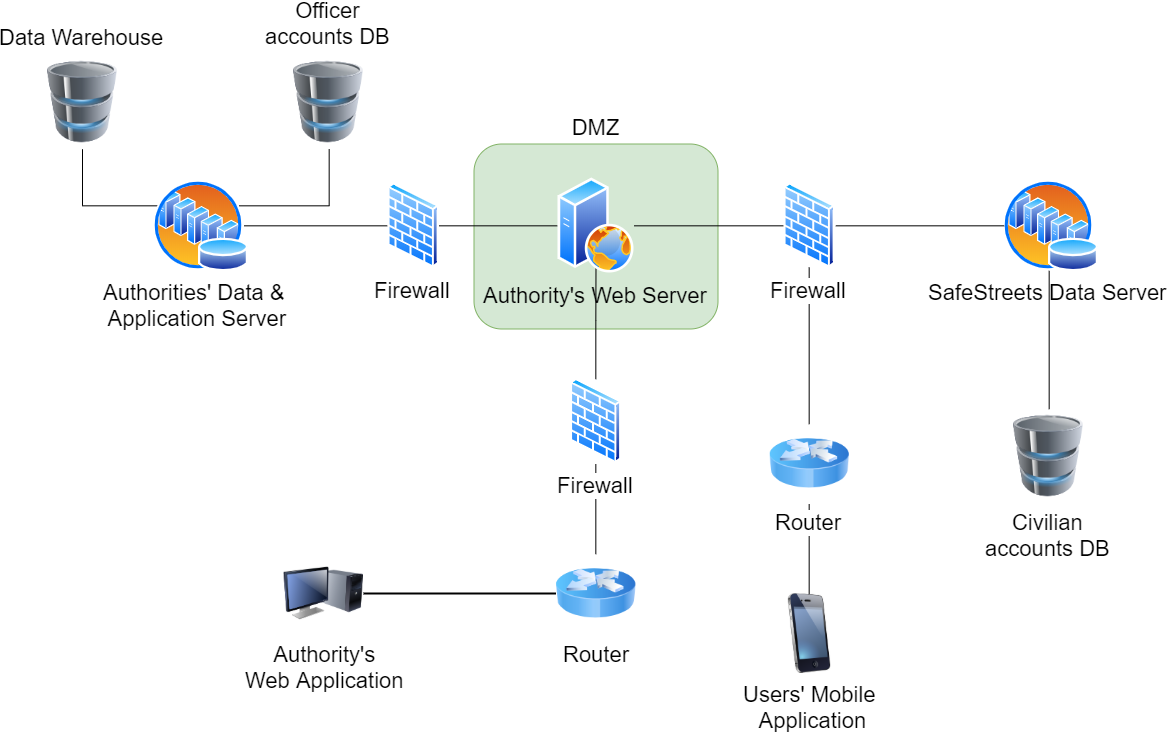
\includegraphics[width=.9\paperwidth,keepaspectratio]{Images/highlevel}
					\end{adjustwidth}
				\caption{High Level Structure with a single Authority and a single User}
			\end{figure}
The three logical layers of the S2B are distributed in a \textbf{three-tier architecture}:
\begin{itemize}
\item \textbf{Presentation layer:} two hard clients:
\begin{itemize}
\item the GUI at the authority's web application is the tool thanks to which the authority's personnel can add officers, receive reports from the users through HTTP calls thanks to a REST architecture embedded in the web server, and validate or invalidate them. It can thus interact directly with the web server, and rarely with the SafeStreets' server to which it sends ban requests. The web server is isolated from the outside by firewalls for increased security and to protect the ADS even if the web server is compromised. The only logic that will be implemented directly at the this client will be the supervised algorithm to recognize plates: this way we can reduce latency, because since the overhead to effectively send a correct plate frame will be pretty heavy, we remove the step to contact the application server and instead execute this function directly at the authorities' location. Anything else will be handled as notifications forwarded to the ADS to limit the computational power used at the authorities' locations.
\item the GUI at the mobile application, which can be used to file reports and send them to the Authority's web server by all users, and which allows officers to check reports and sign automated tickets (and also receives slightly different updates which
include sensitive data to be made unreadable by civilians). 
\end{itemize}
Moreover, both clients must be able to "unpack" the received updates' representations into a format understandable to the user.
\item \textbf{Application layer:} the hypermedia at the mobile application moves from a state to another thanks to the updates received by the authorities' web servers (which are themselves sent to the authorities by the ADS, and then are periodically spread to the clients in the network). While the web server constitutes an interface protected by a DMZ (to isolate it from the ADS) which clients are forced to invoke when applicative functions are needed, the ADS hosts the update producing and ticket emission functionalities. It is important to denote the fact that since every Authority owns a web server, calls received from the mobile units can be handled by any of the authorities for load balancing.  Thus we can say that both the Web server located at the authorities' location and the applicative functions of the ADS constitute this layer. 
\item \textbf{Data layer:} three instances where data access is needed:
\begin{itemize}
\item for managing the civilian accounts and bans, at the SafeStreets server;
\item for managing the officer accounts, at the ADS;
\item for reading and writing historical data about reports in the data warehouse, again at the ADS;
Therefore we can say that application and data services are "partially merged" as the ADS hosts both an application and a data server.
\end{itemize}
\end{itemize}

It is important to notice how the ADS could be implemented in a \texttt{RAPS architecture} where multiple ADS each own a single microservice, for example a server could handle ticket emission, another one officer accounts, and another one update mining and spreading. Another configuration could be assigning an ADS for each authority. 
Web Servers are installed at the authority's location, one for each authority, to better serve nearby mobile units and balance loads, especially in big cities.
The SafeStreet servers could be arranged in a \texttt{RACS architecture} to handle requests from great numbers of civilians.
In some settings such as small towns a lightweight version of the architecture could be employed by running the web server directly in the same machine where the Authority's client is running instead of a standalone device, thus making it a two-tier architecture since the web server wouldn't be separed from the presentation layer anymore.


\newpage
\subsection{Component view}
\subsubsection{High Level Component Diagram}
The following diagrams illustrate the system components and the interfaces through which they interact to fullfil their functionalities. The diagram is focused on the application tier, so the remaining tiers (the presentation tier and the data tier) are shown as black-box.
First we highlight a distinction between Client side and Server side:
\begin{itemize}
\item The Client side is composed by two components, \textit{Web Application} and \textit{Mobile Application}. The first is referred to the Authorities client, latter to the User client (Civilian and Officer).
\item The Server side is composed of three main components: \textit{Authorities Web Services} manages the authorities client, through the \textit{AuthoritiesWebServices} interface server-side; the other two services are the \textit{Civilian Mobile Services} and the \textit{Officer Mobile Services} that manage  the \textit{Mobile Application} from two distinct interfaces.
\end{itemize}
\begin{figure}[H]
		\centering
			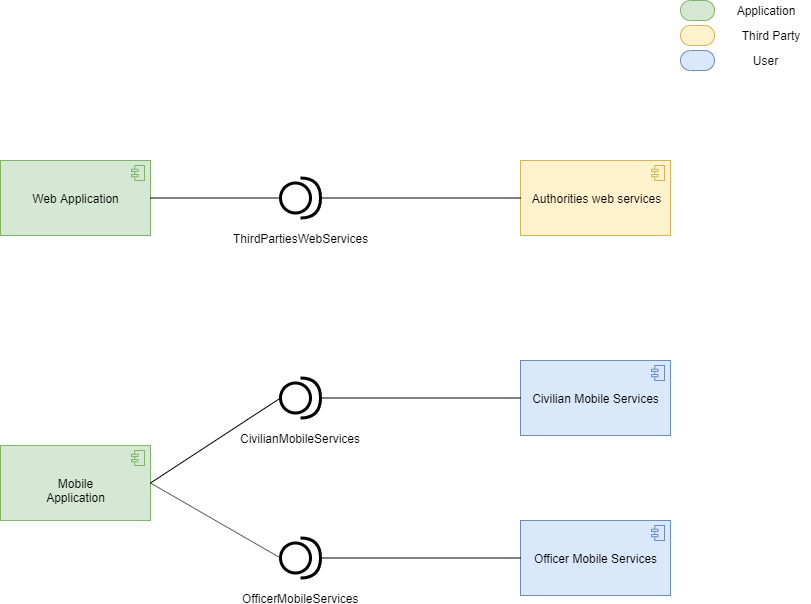
\includegraphics[width=1.0\linewidth]{Images/ComponentDiagram}
		\caption{Component diagram}
\end{figure}

\subsubsection{Civilian Mobile Services Projection}
Civilian Mobile Services subsystem is made of four components: Report Module, Update Module, Data Manage Module and Civilian Authentication Module.
These components provide the Mobile Application the following interfaces: ReportHandler, UpdateHandler, DataManager and AuthenticationHandler. The Modules also communicate with the map, gps services and two DBMS; the first one allows to collect the mined data about reports in the data warehouse, the latter manages user accesses of any form.
\begin{figure}[H]
				\centering
					\begin{adjustwidth}{-25mm}{-25mm}
					        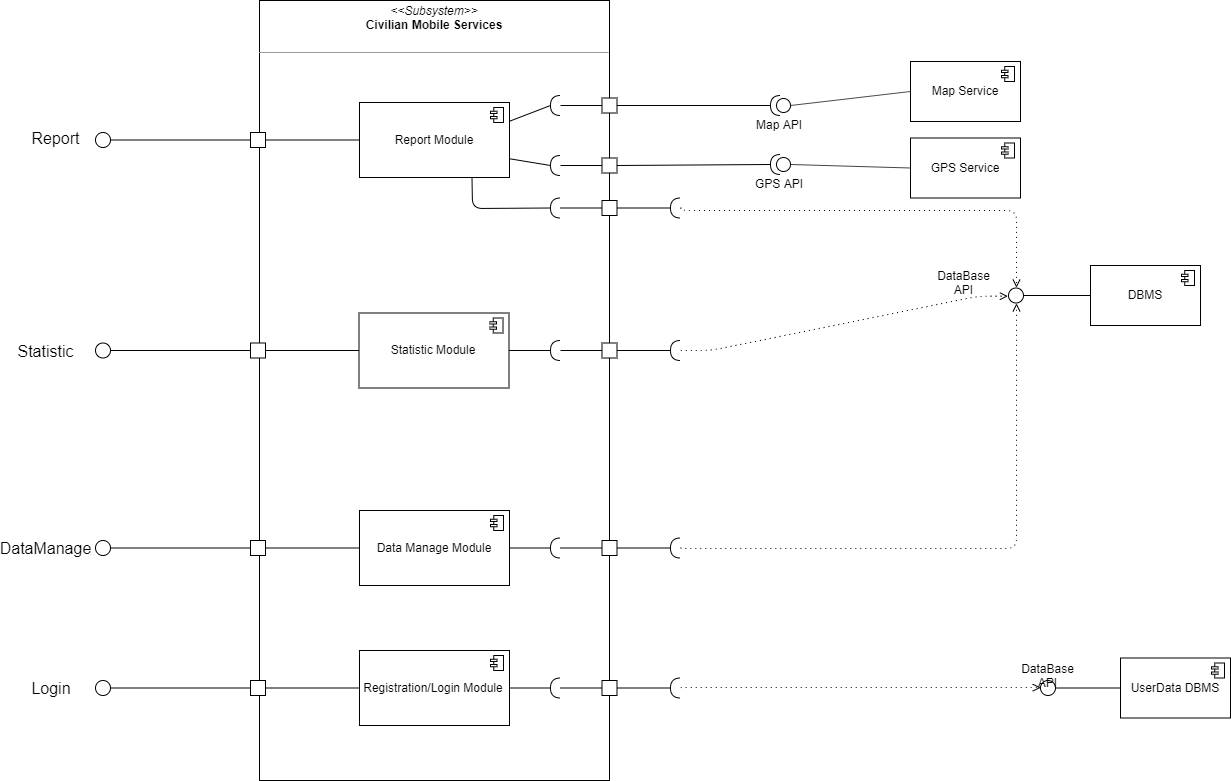
\includegraphics[width=0.9\paperwidth]{Images/CivilianMobileServicesProjection}
					\end{adjustwidth}
			\end{figure}
\textbf{Module Functionalities}
\begin{itemize}
	\item \texttt{Report Module}: this module manages the reports done by Civilians and their sending to the Authority's Web server. It will allow the user to take photos of the violation, enter a description of it, timestamp it and attach geolocation coordinates thanks to the GPS API, and also handle all the communication needed for the plate recognition algorithm to work.
	\item \texttt{Update Module}: this module handles the receiving and visualizing of the mined data about HFVZs, through the Map API.
	\item \texttt{Data Manager Module}: this module allows civilians to manage their personal data (for instance changing their e-mail address or password).
	\item \texttt{Civilian Authentication Module}: this module handles the registration and login requests by civilians, and thus providing the effects of an eventual ban.
\end{itemize}
\newpage
\subsubsection{Officer Mobile Services Projection}
Officer Mobile Services subsystem is an enriched version of the civilian one to accomodate the advanced functions accessible to officers. It is made of four components: Report Module, Update Module, Check Report Module and Officer Authentication Module.
The Report Module works in the same way as the civilian mobile services, while the Update Module possesses quite a few different features to assist the officer. The Check Report Module manages the practice of checking violations by the officer
which might eventually result in a ticket being compiled. The Officer Authentication Module communicates with the Authorities Web Server and not with the SafeStreets server because officer data is kept in the ADS. 
\begin{figure}[H]
				\centering
					\begin{adjustwidth}{-25mm}{-25mm}
					        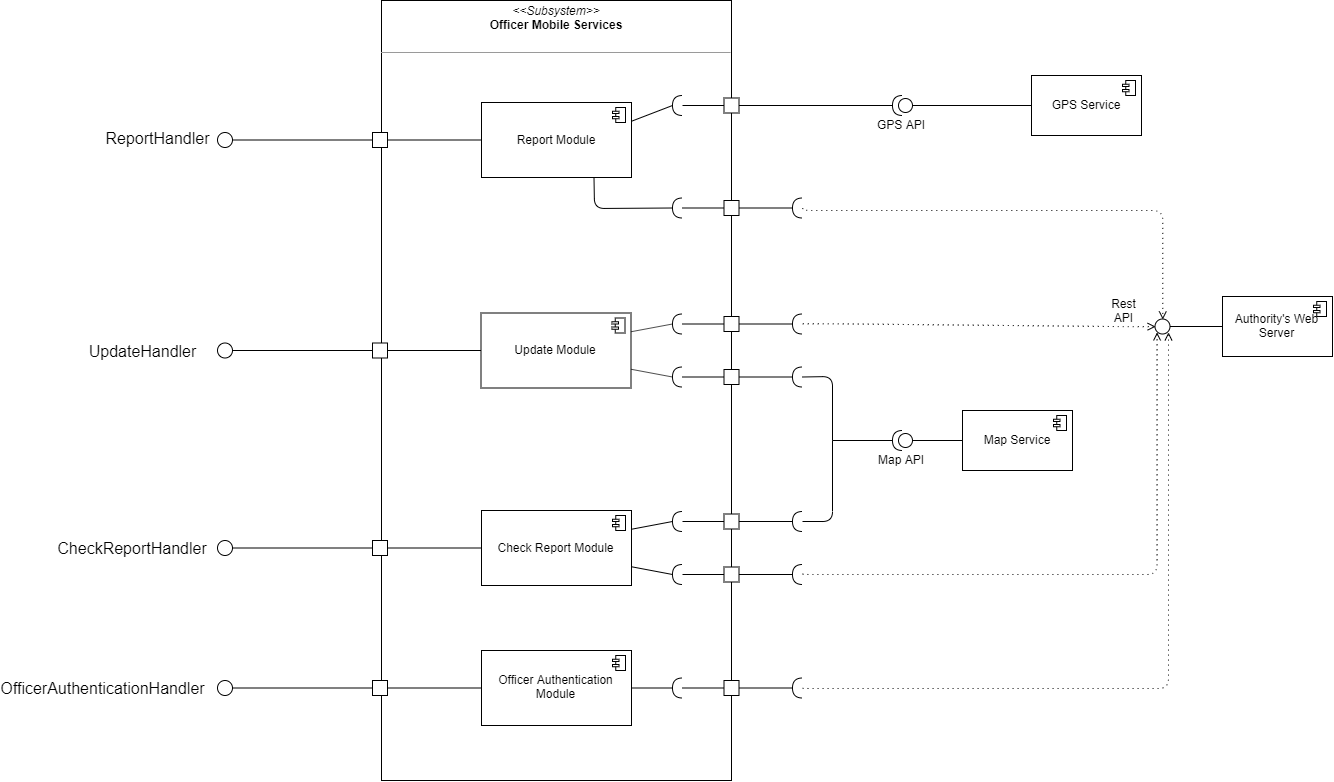
\includegraphics[width=0.9\paperwidth]{Images/OfficerMobileServicesProjection}
					\end{adjustwidth}
			\end{figure}
\textbf{Module Functionalities}
Pretty much the same as the Civilian Mobile Services:
\begin{itemize}
	\item \texttt{Report Module}: works in the same way as the Civilian's one, as officers will also be able to report violations.
	\item \texttt{Update Module}: just as the Civilian's one, but enriched with more updates that should only be accessible to law enforcement agents, such as the most egregious offenders list, newly added reports to the map, etc.
	\item \texttt{Check Report Module}: this module allows the officers to confirm the presence of a violation (and the correctness of the plate shown in the report) and enter a secret PIN to allow the emission of a ticket.
	\item \texttt{Officer Authentication Module}: this module handles the registration and login requests by officers.

\end{itemize}
\newpage
\subsubsection{Authorities Web Services Projection}
The Authorities Web Services are carried out by the Web Server and the ADS, which implements most functions of the application. Five Modules will be implemented to fulfill every functionality: Validation Report, Authority Update, Officer Registration, Officer Authentication, Ticket Emission. Web Server and ADS are strongly intertwined to provide the functionalities which all the three actors' clients need: the web server is in fact an interface which provides a layer for communication for the clients to interact with the ADS, for enhanced security, as every HTTP call which eventually has to reach the ADS to execute some logic has to pass through the web server at some authority's location.
\begin{figure}[H]
				\centering
					\begin{adjustwidth}{-25mm}{-25mm}
					        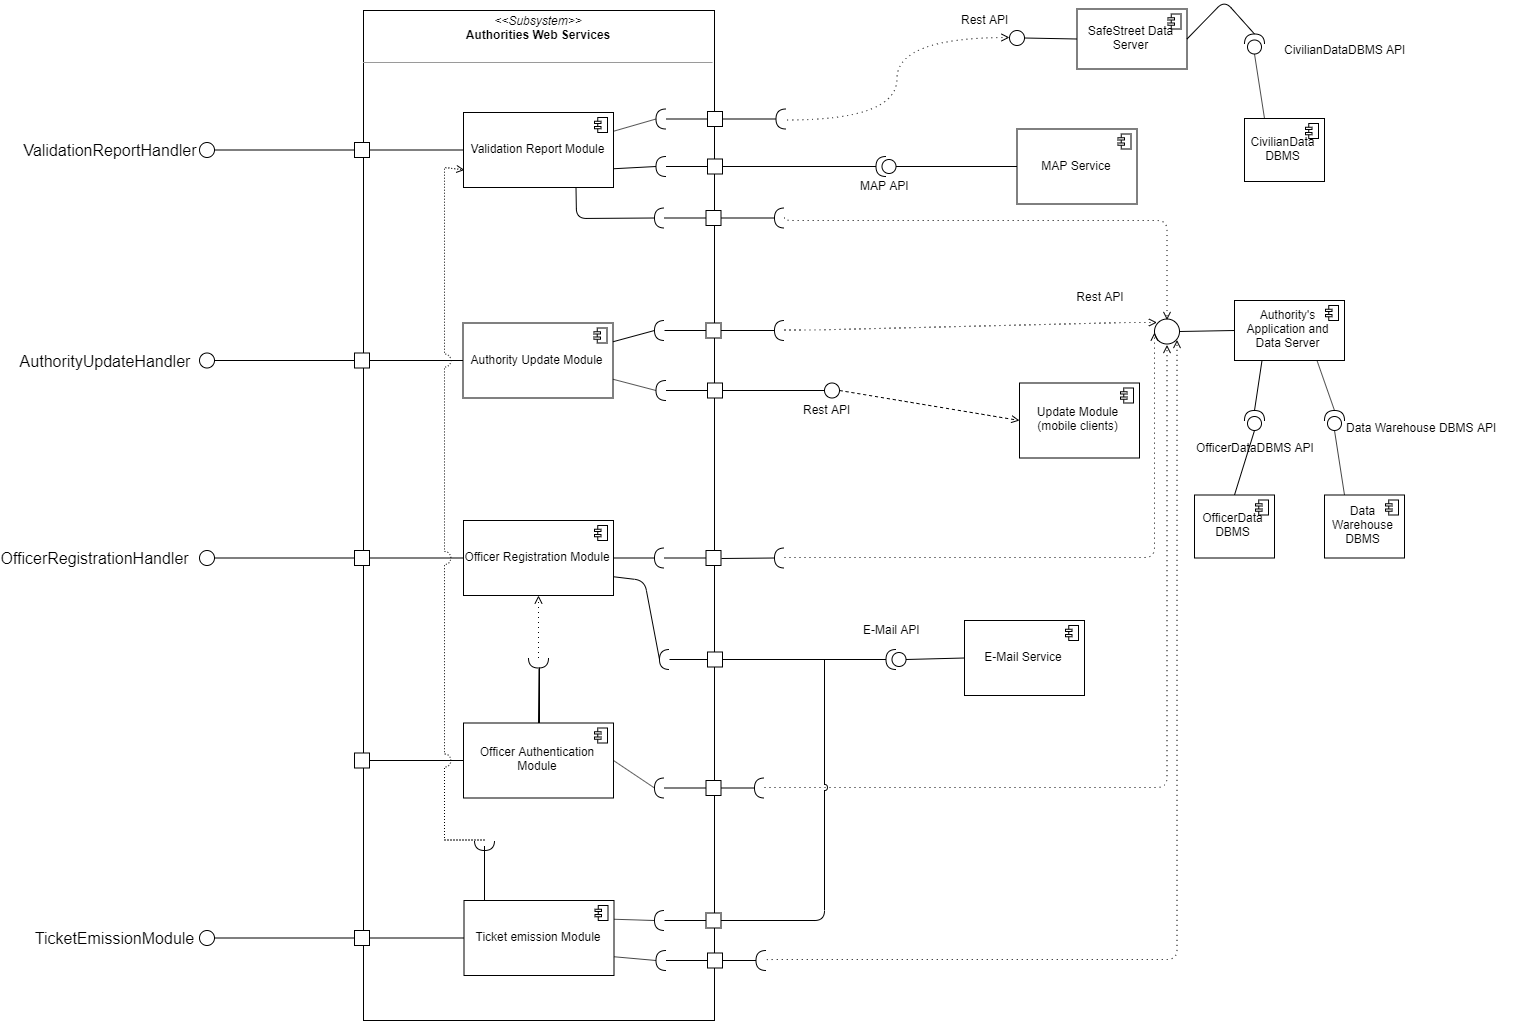
\includegraphics[width=0.9\paperwidth]{Images/AuthoritiesServicesProjection}
					\end{adjustwidth}
			\end{figure}
\textbf{Module Functionalities}
\begin{itemize}
	\item \texttt{Validation Report Module}: this module handles the functionality for validating reports by the authority's personnel and the subsequent adding to the DW.  Also the issuing of bans which is performable while invalidating reports.
	\item \texttt{Authority Update Module}: this module not only handles the receiving of updates by the ADS at the web server location (the updates are the same received by the officers, plus the list of currently active officers), but also the mining which will be run in the ADS by periodically querying the DW to retrieve the data which will be packed to form the updates, that will be sent to the web servers and spread by them to the mobile units.
	\item \texttt{Officer Registration Module}: allows the authority to add new officers, communicating the addition both to the officer via mail and to the ADS. Also manages the first insertion of the secret pin by the officer.
	\item \texttt{Officer Authentication Module}: this module authenticates the officers' login requests from the Officer Authentication Module of the Officer Services, and the pin insertion from the Check Report module.
\end{itemize}
\newpage
\subsubsection{Complete Component Diagram}
This diagram shows the interactions between all the subsystems of the application for better clarity. The presence of multiple REST APIs instead of a single comprehensive one has been modeled to show the different connections between modules without ambiguity.
\begin{figure}[H]
				\centering
					\begin{adjustwidth}{-25mm}{-25mm}
					        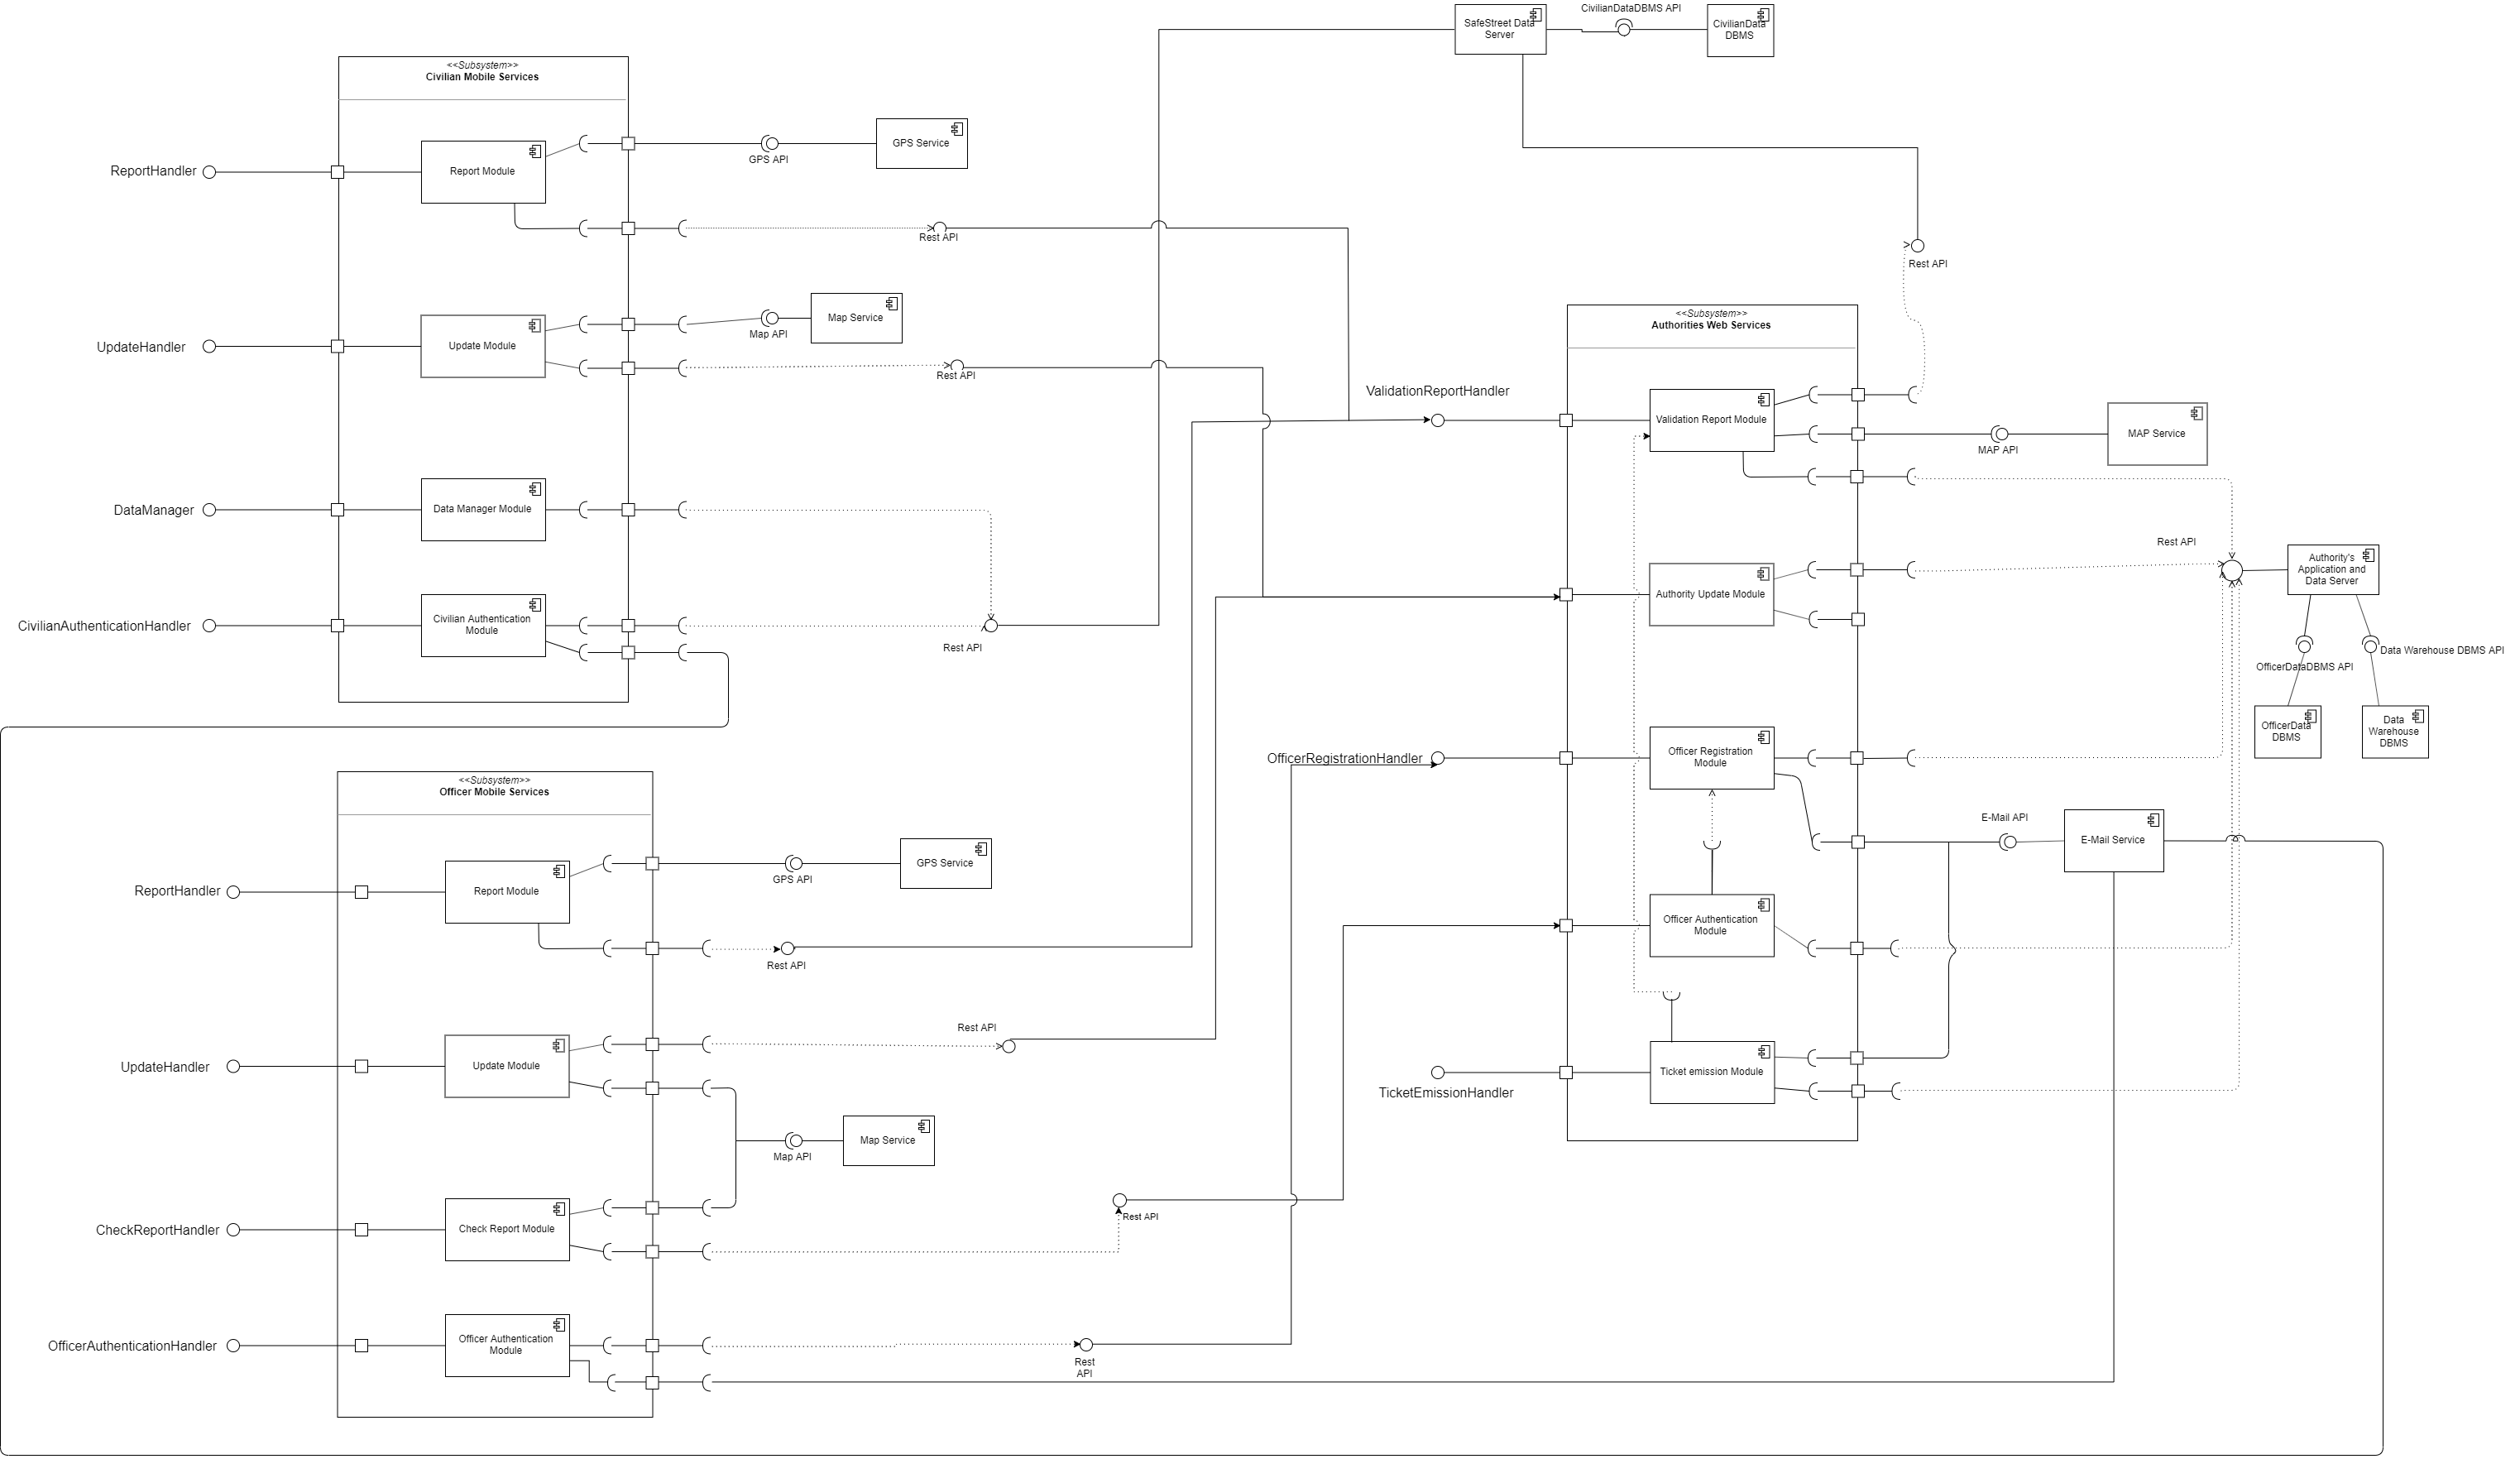
\includegraphics[width=0.95\paperwidth]{Images/OverallComponent}
					\end{adjustwidth}
			\end{figure}
\newpage
\subsection{Deployment view}
The architecture of the S2B, as shown in the component view paragraph, will be arranged in three tiers:
\begin{itemize}
\item \textbf{First tier:} is composed of the smartphones of the civilians and officers which run the mobile application, both in Android and iOS operative systems, and by the computer located at the Authority. All these clients communicate with the web server via HTTP thanks to a REST architecture, while mobile units can log in as civilians contacting the SafeStreets server.
\begin{figure}[H]
				\centering
					        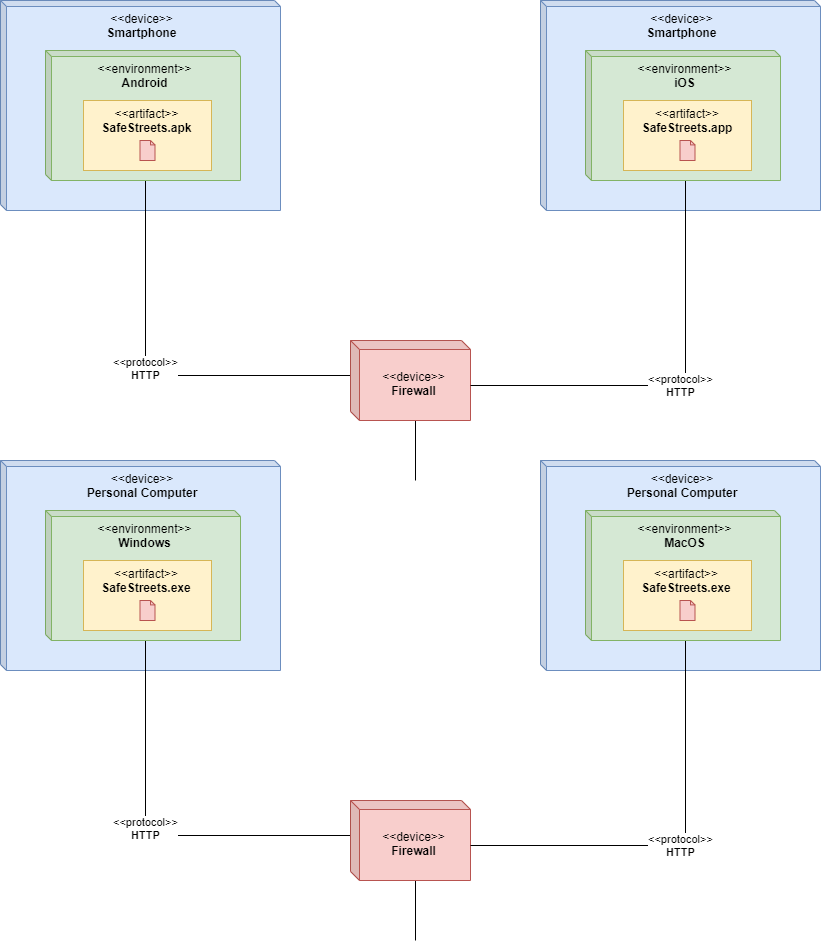
\includegraphics[width=0.6\paperwidth]{Images/firstTier}
			\end{figure}
\newpage
\item \textbf{Second tier:} is made of the Web Server which acts as a layer of communication for clients which want to interact with the ADS. We chose Apache Tomcat as web server as it is efficient and easy to implement through Spring Boot.
\begin{figure}[H]
				\centering				
					        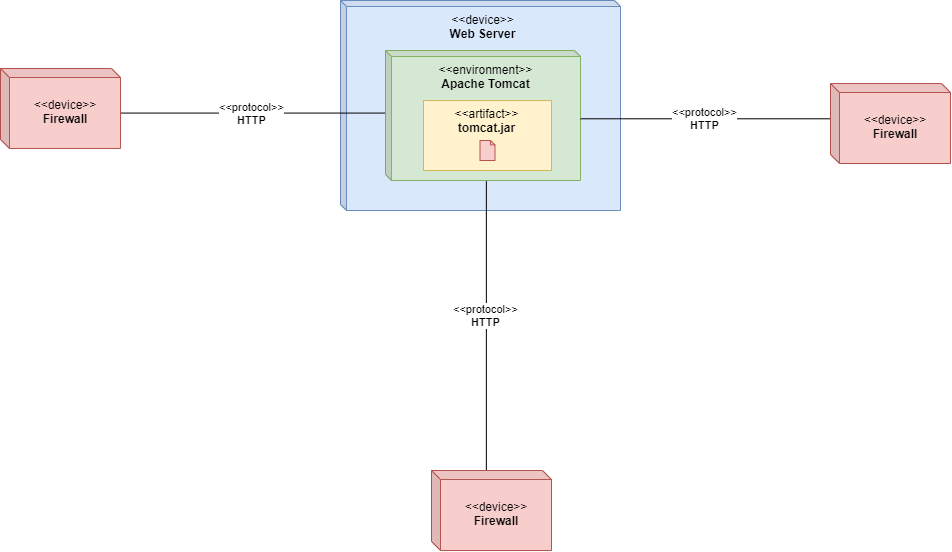
\includegraphics[width=0.7\paperwidth]{Images/secondTier}
			\end{figure}
\newpage
\item \textbf{Third tier:} the ADS with its application server and data servers, which communicate with the Officer Accounts database and with the Data Warehouse whose data is accessed through Hibernate which is again made easily interoperable with Spring Boot. The same implementation is used by the SafeStreet server which manages civilian accounts. We chose WildFly for the application servers because like Tomcat it provides a well documented and easily implementable framework.
\begin{figure}[H]
				\centering				
					        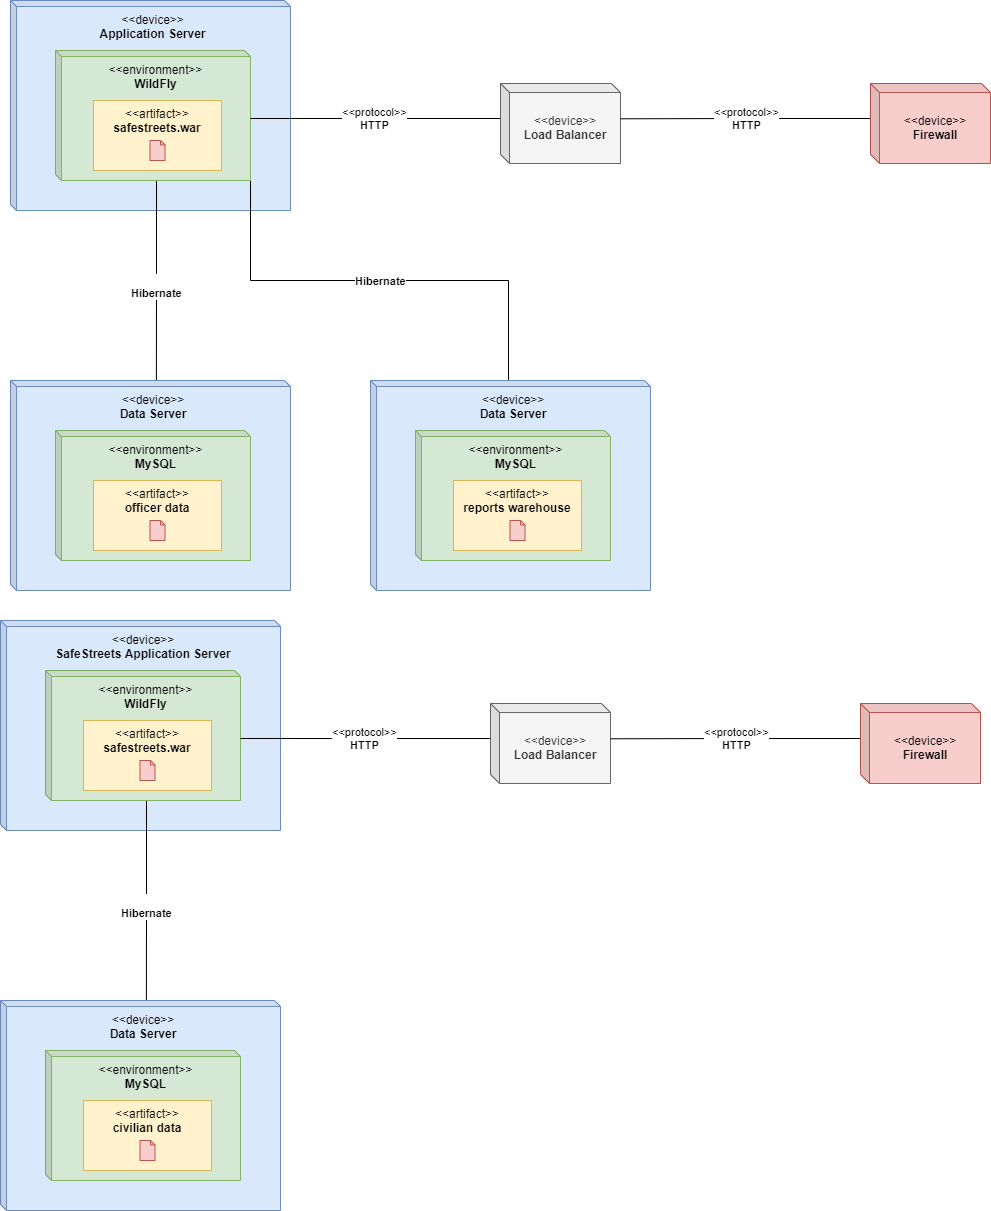
\includegraphics[width=0.6\paperwidth]{Images/thirdTier}
			\end{figure}
\end{itemize}
\newpage
This diagram represents the deployment view for the entire system:
\begin{figure}[H]
\begin{adjustwidth}{-25mm}{-25mm}
				\centering				
					        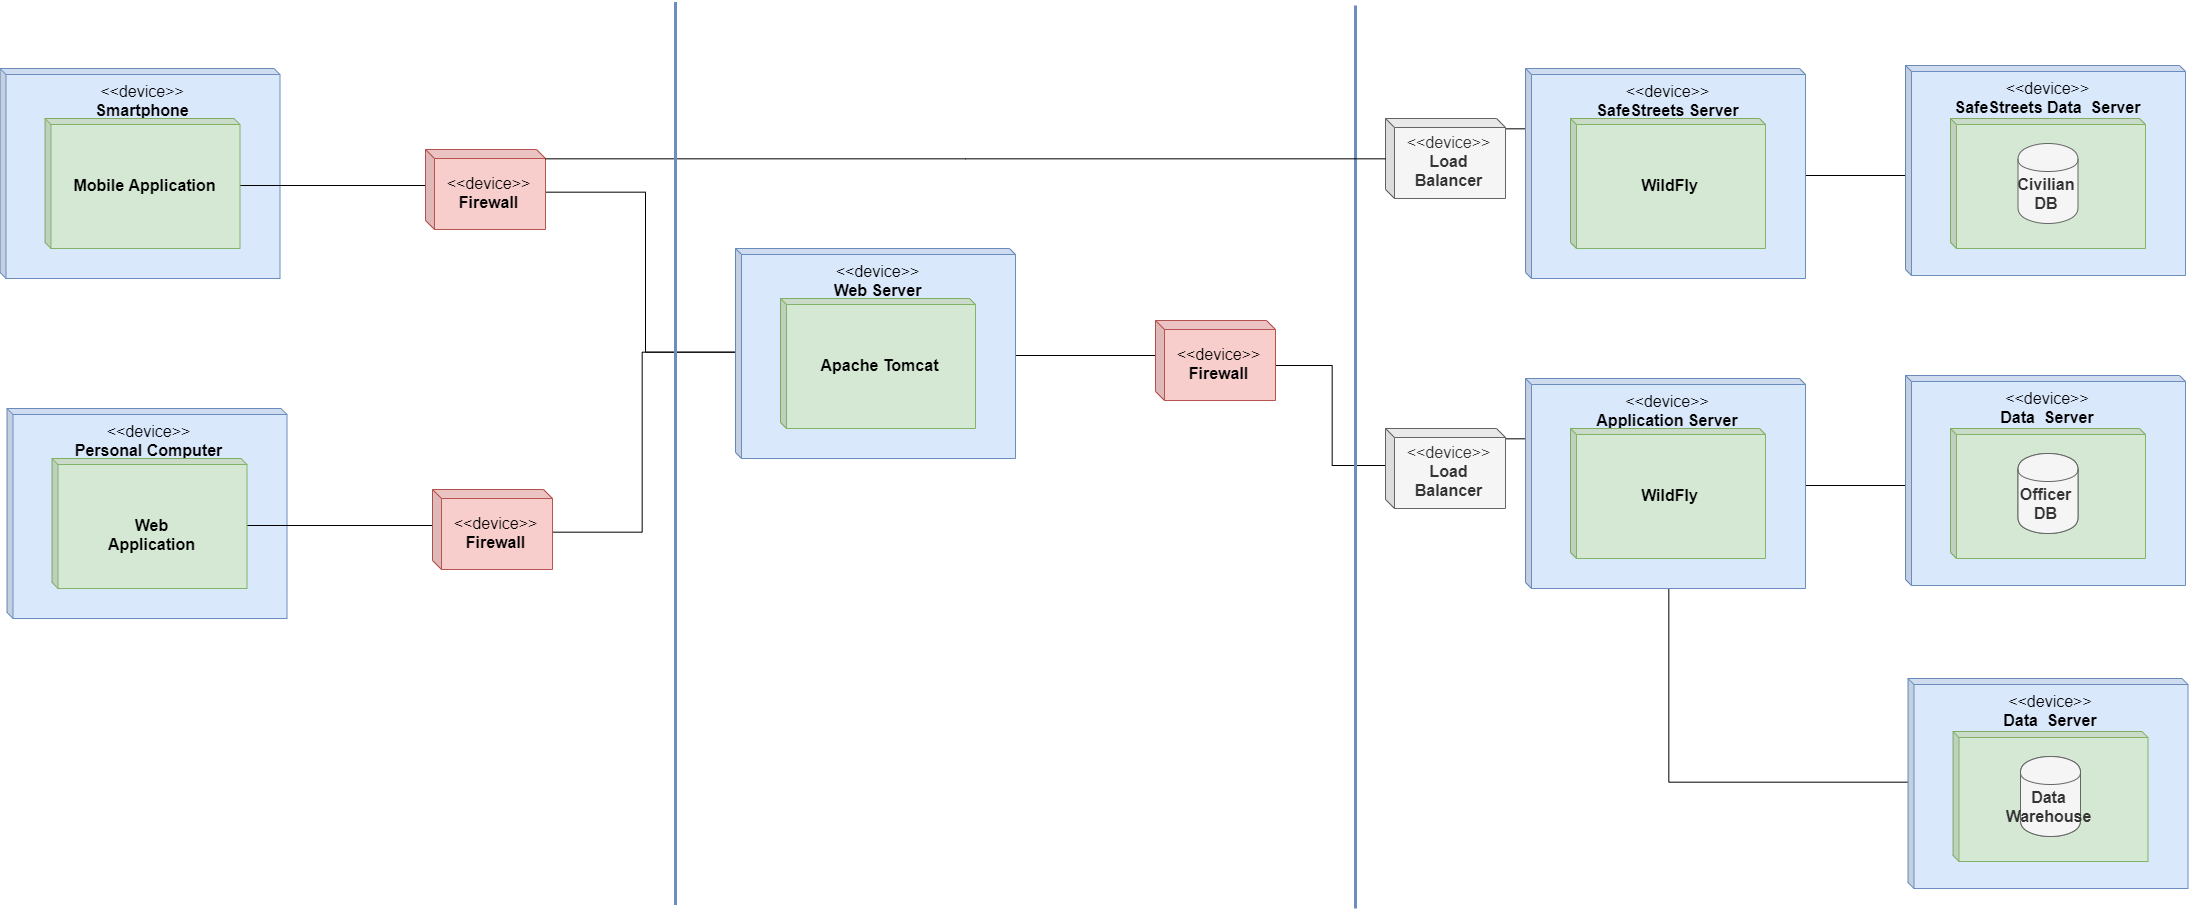
\includegraphics[width=0.9\paperwidth]{Images/deploymentView}
\end{adjustwidth}
			\end{figure}
\subsection{Runtime view: You can use sequence diagrams to describe the way components interact to accomplish specific tasks typically related to your use cases}
\subsection{Component interfaces}
\subsubsection{External Interfaces}
SafeStreets will make use of some Application Programming Interfaces to simplify the implementation, since these components are largely used and compatible with the majority of the devices currently on the market:
\begin{itemize}
\item \texttt{Maps API} to have a visual representation of users' reports and HFVZs, to help Officers in finding a report that coud be confirmed or rejected. For our purpose the Google Maps API is perfectly suitable, since it can be embedded in both Android and iOS applications.
\item \texttt{GPS API} to geolocate the reports made by users and  avoid the possibility of forging the location, which could happen if users manually enters it. GPS will also provide the application with precise timestamps for the reports.
\item \texttt{REST API} every distributed component will be provided with a REST API, especially mobile clients will exploit it to interact with the web server at the Authority's location, which is the only layer visible to them. Also the SafeStreets data server's services and the ADS's will be invokable through a REST interface. Spring Boot, which uses Apache Tomcat as a web server, could be used as a versatile, easy to implement solution to build a functioning REST architecture across all subsystems.
\item \texttt{DBMS API} will be used to read and write all the database components:
\item one at the SafeStreets server which manages civilian accounts;
\item one DW at the ADS location which holds records for all reports ever compiled and is queried to create the updates;
\item another one at the ADS location which manages officer accounts.
We will use MySQL as the DBMS, which will be manipulated directly from the software from the Hibernate API which can be easily configured to work with Spring Boot for simplicity and performance.
\item \texttt{E-Mail API} to send an Email to the officers added to the SafeStreets project and to send the compiled ticket to the VLA. 
\end{itemize}
\subsection{Selected architectural styles and patterns: Please explain which styles/patterns you used, why, and how}
\subsection{Other design decisions}
\section{USER INTERFACE DESIGN: Provide an overview on how the user interface(s) of your system will look like; if you have included this part in the RASD, you can simply refer to what you have already done, possibly, providing here some extensions if applicable.}
\section{REQUIREMENTS TRACEABILITY}
In the following table it is highlighted the link between the functional requirements stated in the RASD and the components listed in the section 2.2.
\begin{center}
\begin{tabular}{| l | l | l |}
	\hline
	\textbf{Requirement} & \textbf{Referring Goal} & \textbf{Component (DD)} \\ \hline
		[R1]: Separate civilian and officer \\ registration and login functionality. & [G1-G5.2] & Officer Registration Module \\ Officer Authentication Module \\ civilian Authentication Module \\ \hline
		[R2]: Data has to be correctly queried\\ server-side everytime, to make sure no\\ duplicate accounts are created \\ or no unregistered visitors log in. & [G1] & Officer Registration Module - Officer Authentication Module - civilian Authentication Module \\ \hline
		[R3]: Send confirmation emails \\within at most one minute after \\the registration confirmation receipt \\(or the new officer being added). & [G1] & Officer Registration Module - civilian Authentication Module\\ \hline
		[R4]: Confirm user registration \\within at most one minute after \\the email link has been clicked. & [G1] & Officer Registration Module - civilian Authentication Module \\ \hline
		[R5]: Force the user to allow \\the S2B to access the device's \\camera and GPS. & [G2] & Report Module - Update Module \\ \hline
		[R6]: Implement a function in the \\authority's client which allows \\personnel to validate or \\invalidate reports. & [G2-G5.1] & Validation Report Module \\ \hline
		[R7]: Implement a supervised learning \\algorithm server-side which scans\\ the multiple frames sent by the\\ user to recognize the license plate. & [G2-G5.1] & Validation Report Module \\ \hline
		[R8]: Automatically discard the report\\ if another one with the same plate \\has been received within an\\ hour to avoid duplicates. & [G2-G5.1] & Validation Report Module \\ \hline
		[R9]: The supervised learning \\algorithm must be accurate at\\ least 99\% of the times. & [G2-G5.1] & Validation Report Module \\ \hline
		[R10]: Acknowledgments from the authority's\\ server must be received within 10 seconds. & [G2] & Validation Report Module \\ \hline
		[R11]: Store the report info in the DW \\everytime it is confirmed to be valid. & [G3] & Authority Update Module \\ \hline
		[R12]: Make the data warehousing and \\processing completely invisible to human\\ actors to avoid manipulations. & [G3] & Authority Update Module \\ \hline
		[R13]: implement functionality which \\allows (through the authority's client) to toggle\\ automatic tickets ON or OFF. & [G4.1] & Ticket Emission Module \\ \hline
		[R14]: force newly logged officers to\\ choose a 5 digit pin to release tickets. & [G4.1] & Officer Registration Module \\ \hline
		[R15]: implement functionality which allows\\ officers' near a report to confirm both\\ the report itself and the ticket\\ emission through the pin. & [G4.1] & Check Report Module - Ticket Emission Module \\ \hline
		[R16]: implement functionality which \\uses report data and the officer's \\signature to compile a ticket and\\ send it to the VLA via email. & [G4.1] & Check Report Module - Ticket Emission Module \\ \hline
		[R17]: update every actor's map with\\ the HFVZs every 30 seconds. & [G4.2] & Update Module - Authority Update Module \\ \hline
		[R18]: update only the authorities' \\and officers' maps with the new reports \\and repeat offenders lists \\in real time. & [G4.2-G6] & Update Module - Authority Update Module \\ \hline
		[R19]: show repetead offenders in \\real time in the authorities' GUI. & [G4.2] & Authority Update Module \\ \hline
		[R20]: Make sure officers can only be\\ added through the Authority's client. & [G5.2] & Officer Registration Module \\ \hline
		[R21]: Officers can only log into \\the app through a combination of \\Badge ID and a password received\\ via email by the Authority. & [G5.2-G5.3] & Officer Registration Module - Officer Authentication Module \\ \hline
		[R22]: Officers can only allow automated\\ ticket emission by entering their secret pin. & [G5.3] & Check Report Module - Ticket Emission Module \\ \hline
		[R23]: Officers are automatically required \\to login every 6 hours and their access data \\can't be autofilled. & [G5.3] & Officer Authentication Module \\ \hline
		[R24]: A ban request can be issued \\through the Authority's client \\after receiving an invalid report. & [G5.4] & Validation Report Module \\ \hline
		[R25]: The S2B must comply with GDPR rules. & [G6] & Data Manager Module \\ \hline
\end{tabular}
\end{center}
\section{IMPLEMENTATION, INTEGRATION AND TEST PLAN: Identify here the order in which you plan to implement the subcomponents of your system and the order in which you plan to integrate such subcomponents and test the integration.}
\section{EFFORT SPENT}
\begin{itemize}
\item {Davide Cocco}
 \begin{center}
			\begin{tabular}{| c | l | c |}
				\hline
				\textbf{Day} & \textbf{Subject} & \textbf{Hours} \\ \hline
				14/11/2019 & High level components & 3 \\ \hline
				19/11/2019 & Component view & 4 \\ \hline
				20/11/2019 & Deployment view & 2 \\ \hline
				Total & & ** \\ \hline
			\end{tabular}
		\end{center}
\item {Marco Gasperini}
\begin{center}
			\begin{tabular}{| c | l | c |}
				\hline
				\textbf{Day} & \textbf{Subject} & \textbf{Hours} \\ \hline
				14/11/2019 & Purpose and Scope & 1 \\ \hline
				19/11/2019 & Component view & 5 \\ \hline
				Total & & ** \\ \hline
			\end{tabular}
\end{center}
\end{itemize}
\section{References}

\end {document}